% 2 章：確率的ボラティリティモデル
% 定義は実装と一致させている：src/sv_vi/logdensity.py（同時密度）、models.py（NumPyro 版）、
% simulate.py（合成データ）、predictive.py（予測分布）。図表は experiments/f1_model_illustration.py が生成。
\section{確率的ボラティリティモデル}\label{sec:model}

本章では、本稿で扱う確率的ボラティリティ（SV）モデルを定義し、その性質を整理する。
\cref{sec:model-data} でデータの単位と記法を定め、\cref{sec:model-basic,sec:model-properties} で基本 SV モデルとその性質（裾の厚さ、ボラティリティ・クラスタリング）を述べる。
\cref{sec:model-leverage,sec:model-t} で二つの拡張（レバレッジ効果、$t$ 分布の誤差）を、\cref{sec:model-prior} で事前分布を示す。
\cref{sec:model-likelihood,sec:model-structure} では、尤度が解析的に書けない理由と、事後分布が持つ構造（三重対角の精度行列）を説明する。
この構造が、\cref{sec:family} で変分族を設計するときの出発点になる。
最後に、推定の実務で重要になるパラメータ化の選択（\cref{sec:model-param}）と、VaR の計算に使う 1 期先の予測分布（\cref{sec:model-predictive}）を述べる。

\subsection{データと記法}\label{sec:model-data}

資産の終値（分割などを調整した価格）を $P_t$ とし、日次の対数リターンを \% 単位で
\[
  r_t = 100\,(\log P_t - \log P_{t-1}), \qquad t = 1, \dots, T
\]
と定義する。本稿のモデルでは、標本平均 $\bar r$ を引いた
\[
  y_t = r_t - \bar r
\]
を観測とする。日次リターンの平均は 0.05\% 程度と、日次の標準偏差（1\% 前後）に比べて十分に小さいので、
平均を定数として事前に除いても推定への影響は小さく、モデルを「散らばりの変動」だけに集中させることができる。
\cref{sec:empirical} のローリング推定では、先読みを避けるため、各時点の推定窓の中だけで平均を計算して除き、翌日のリターンにも同じ平均を使う。

\% 単位を使うのは、数値を扱いやすい範囲に収めるためである。
後で導入する対数ボラティリティ $h_t$ を使うと、日次リターンの条件付き標準偏差は $\exp(h_t/2)$（\%）、
年率換算のボラティリティは $\sqrt{252}\,\exp(h_t/2)$（\%）になる（1 年を 252 営業日とする）。
例えば $h_t = 0$ は日次 1\%、年率約 15.9\% に対応し、$h_t = 1$ なら日次 1.65\%、年率約 26\% である。
生の対数リターン（小数）を使うと $h_t$ は $-9$ 前後の値をとり、同じ事前分布でも意味が変わってしまう。
事前分布の妥当性は単位に依存するので、本稿の事前分布（\cref{sec:model-prior}）は \% 単位を前提に設定している。

記法をまとめておく。$y_{1:T} = (y_1, \dots, y_T)$ のように添字の範囲で列を表し、紛れがなければ単に $y$、$h$ と書く。
$\Normal(m, v)$ は平均 $m$、分散 $v$ の正規分布、$\Normal(x \mid m, v)$ はその密度を $x$ で評価した値である。
モデルの大域パラメータをまとめて $\theta$ と書く。基本 SV モデルでは $\theta = (\mu, \phi, \sigma)$、レバレッジ SV では $\rho$ が、$t$ 誤差の SV では $\nu$ が加わる。

\subsection{基本 SV モデル}\label{sec:model-basic}

基本 SV モデル \parencite{taylor1986,jacquier1994,kim1998} は次の二つの式からなる。
\begin{align}
  y_t &= \exp(h_t/2)\,\varepsilon_t, & \varepsilon_t &\sim \Normal(0, 1), & t &= 1, \dots, T, \label{eq:sv-obs}\\
  h_{t+1} &= \mu + \phi\,(h_t - \mu) + \sigma\,\eta_t, & \eta_t &\sim \Normal(0, 1), & t &= 1, \dots, T-1, \label{eq:sv-state}\\
  h_1 &\sim \Normal\!\left(\mu,\ \frac{\sigma^2}{1-\phi^2}\right). \label{eq:sv-init}
\end{align}
ここで $\varepsilon_t$ と $\eta_s$ はすべての $t, s$ について互いに独立とする（独立でない場合が次節以降のレバレッジ SV である）。

\cref{eq:sv-obs} は\textbf{観測方程式}であり、リターン $y_t$ が、平均 0、分散 $\exp(h_t)$ の正規分布に従うことを表す。
$h_t$ は日次分散の対数（対数ボラティリティ）であり、観測されない\textbf{潜在変数（状態変数）}である。
\cref{eq:sv-state} は\textbf{状態方程式}であり、$h_t$ が平均 $\mu$ のまわりを変動する 1 次の自己回帰過程（AR(1) 過程）に従うことを表す。
\cref{eq:sv-init} は初期値 $h_1$ を AR(1) 過程の定常分布から始めることを意味し、これにより $h_1, h_2, \dots$ はすべて同じ周辺分布 $\Normal(\mu, \sigma^2/(1-\phi^2))$ を持つ。

三つのパラメータの意味は次のとおりである。
\begin{itemize}
  \item $\mu \in \mathbb{R}$：対数ボラティリティの長期的な水準。$h_t$ はショックを受けても、長い目で見ると $\mu$ のまわりに戻ってくる。
    \% 単位のリターンでは、$\mu$ がおよそ $-1$〜$2$（日次 0.6〜2.7\%）の範囲にあることが多い。
  \item $\phi \in (-1, 1)$：対数ボラティリティの持続性。$h_t - \mu$ が 1 日で $\phi$ 倍になって残る。
    株価指数の日次データでは $0.95$〜$0.99$ 程度の値が推定されることが多い。$|\phi| < 1$ は $h_t$ が定常であるための条件である。
  \item $\sigma > 0$：対数ボラティリティそのものの変動の大きさ（ボラティリティのボラティリティ）。
    $\sigma$ が大きいほど、ボラティリティは日々大きく揺れ動く。
\end{itemize}

このモデルは\textbf{状態空間モデル}の一種とみなせる。
$h_{1:T}$ はマルコフ連鎖であり、$h_{t+1}$ の分布は $h_t$ だけで決まる。
また、$h_{1:T}$ をすべて与えると、$y_t$ どうしは互いに独立で、$y_t$ の分布は同じ日の $h_t$ だけで決まる。
したがって同時分布は
\begin{equation}
  p(y_{1:T}, h_{1:T} \mid \theta)
  = \underbrace{p(h_1 \mid \theta) \prod_{t=1}^{T-1} p(h_{t+1} \mid h_t, \theta)}_{p(h_{1:T} \mid \theta)}
    \;\underbrace{\prod_{t=1}^{T} p(y_t \mid h_t)}_{p(y_{1:T} \mid h_{1:T})}
  \label{eq:sv-joint}
\end{equation}
と、「AR(1) 過程の事前分布」と「各日の観測の尤度の積」に分解できる。
各日の観測の対数尤度は
\begin{equation}
  \log p(y_t \mid h_t) = -\frac{1}{2}\log(2\pi) - \frac{h_t}{2} - \frac{y_t^2}{2}\,e^{-h_t}
  \label{eq:sv-loglik}
\end{equation}
である。この分解は、後で事後分布の構造を調べるとき（\cref{sec:model-structure}）にも、変分族を設計するとき（\cref{sec:family}）にも中心的な役割を果たす。

GARCH 型モデルとの違いをもう一度確認しておく。
GARCH(1,1) では、条件付き分散 $\sigma_t^2$ は前日までのリターンから決定論的に計算でき、$y_1, \dots, y_{t-1}$ を知れば $\sigma_t^2$ は確定する。
これに対して SV モデルでは、$h_t$ は過去のリターンを知っても確定せず、確率的なショック $\eta_{t-1}$ の分だけ不確実性が残る。
つまり SV モデルでは、ボラティリティは「観測から計算する量」ではなく「観測から\textbf{推測する}量」であり、その推測の不確実性も含めて扱う必要がある。
この違いが、表現力の高さ（\cref{sec:model-properties}）と、推定の難しさ（\cref{sec:model-likelihood}）の両方の源になっている。

\subsection{基本 SV モデルの性質}\label{sec:model-properties}

基本 SV モデルは単純な形をしているが、金融リターンの代表的な性質である\textbf{裾の厚さ}と\textbf{ボラティリティ・クラスタリング}を再現する。
ここでは、それを定常状態でのモーメントの計算で確認する。
導出は、$h_t$ が正規分布に従うとき $\E[e^{a h_t}] = \exp(a\mu + a^2 s^2/2)$ となること（対数正規分布のモーメント）だけを使う。

\paragraph{定常分布}
$h_t$ の定常分布は $\Normal(\mu, s^2)$ であり、その分散は
\[
  s^2 = \frac{\sigma^2}{1-\phi^2}
\]
である。$s$ は「対数ボラティリティが長期的にどの程度の幅で動くか」を表す。
$\phi$ が 1 に近いと、$\sigma$ が小さくても $s$ は大きくなる。
例えば $\phi = 0.97$、$\sigma = 0.15$ では $s \approx 0.62$ であり、日次の標準偏差 $\exp(h_t/2)$ は定常分布の 95\% の範囲で
$\exp(\pm 1.96 \times 0.62 / 2) \approx 0.55$〜$1.83$ 倍の幅で変動する。

\paragraph{分散と尖度}
$\varepsilon_t$ と $h_t$ が独立であることから、
\[
  \E[y_t^2] = \E[e^{h_t}]\,\E[\varepsilon_t^2] = e^{\mu + s^2/2}, \qquad
  \E[y_t^4] = \E[e^{2h_t}]\,\E[\varepsilon_t^4] = 3\,e^{2\mu + 2s^2}
\]
となり、$y_t$ の（周辺分布の）尖度は
\begin{equation}
  \kappa = \frac{\E[y_t^4]}{\E[y_t^2]^2} = 3\,e^{s^2} > 3
  \label{eq:sv-kurtosis}
\end{equation}
である。
各日の条件付き分布は正規分布であっても、分散が日によって変わるため、それらを混ぜ合わせた周辺分布は正規分布（尖度 3）よりも裾が厚くなる。
これは、\cref{sec:intro-models} で触れた混合分布仮説 \parencite{clark1973} の数式による表現である。
なお、$\E[y_t^2] = e^{\mu + s^2/2}$ であるから、無条件の日次分散は $e^{\mu}$ よりも少し大きい。
$\mu$ は「典型的な日」の対数分散であり、平均的な分散そのものではない点に注意が要る。

\paragraph{二乗リターンの自己相関}
$k \geq 1$ について、$h_t$ と $h_{t+k}$ の共分散は $\phi^k s^2$ であるから、
\[
  \mathrm{Cov}(y_t^2, y_{t+k}^2) = \E[e^{h_t + h_{t+k}}] - \E[e^{h_t}]^2 = e^{2\mu + s^2}\left(e^{\phi^k s^2} - 1\right),
  \qquad
  \mathrm{Var}(y_t^2) = e^{2\mu + s^2}\left(3 e^{s^2} - 1\right)
\]
となり、二乗リターンの自己相関は
\begin{equation}
  \mathrm{Corr}(y_t^2, y_{t+k}^2) = \frac{e^{\phi^k s^2} - 1}{3 e^{s^2} - 1}
  \label{eq:sv-acf}
\end{equation}
で与えられる。
リターン $y_t$ 自体は互いに無相関（$\E[y_t y_{t+k}] = 0$）であるのに、二乗リターンは正の自己相関を持つ。
これがボラティリティ・クラスタリングである。
$s^2$ が小さいときは $e^{x} - 1 \approx x$ より $\mathrm{Corr}(y_t^2, y_{t+k}^2) \approx \phi^k s^2 / (3e^{s^2} - 1)$ であり、自己相関は $\phi^k$ の速さで減衰する。
GARCH(1,1) では二乗リターンの自己相関が $(\alpha + \beta)^k$ の速さで減衰することが知られており、\textbf{SV モデルの $\phi$ は GARCH の $\alpha + \beta$ に相当する持続性の指標}と理解できる。

\paragraph{ボラティリティのショックの半減期}
対数ボラティリティに加わったショックは、平均的には 1 日ごとに $\phi$ 倍に減衰するので、ショックが半分になるまでの日数（半減期）は
\[
  \tau_{1/2} = \frac{\log 0.5}{\log \phi}
\]
である。$\phi = 0.97$ なら約 23 日、$\phi = 0.99$ なら約 69 日、$\phi = 0.8$ なら約 3 日になる。
リスク管理の現場の言葉に直せば、「ボラティリティが急上昇した後、平常に戻るまでにどの程度かかるか」を決めるのが $\phi$ である。

\cref{fig:sv-illustration} に、合成データの標準シナリオ（$\mu = 0$、$\phi = 0.97$、$\sigma = 0.15$。\cref{sec:synthetic} で使う）から生成した 1,000 日分のリターンと、その真の年率ボラティリティを示す。
ボラティリティの高い時期と低い時期が交互に現れ、それに応じてリターンの振れ幅が変わる様子が分かる。
パネル (c) は、二乗リターンの自己相関の理論値 \cref{eq:sv-acf} を三つのシナリオについて描き、標準シナリオについては 20 万日分の合成データから計算した標本自己相関を重ねたものである。
標本値は理論値によく一致しており、持続性 $\phi$ が自己相関の減衰の速さを決めていることが読み取れる。

\begin{figure}[tbp]
  \centering
  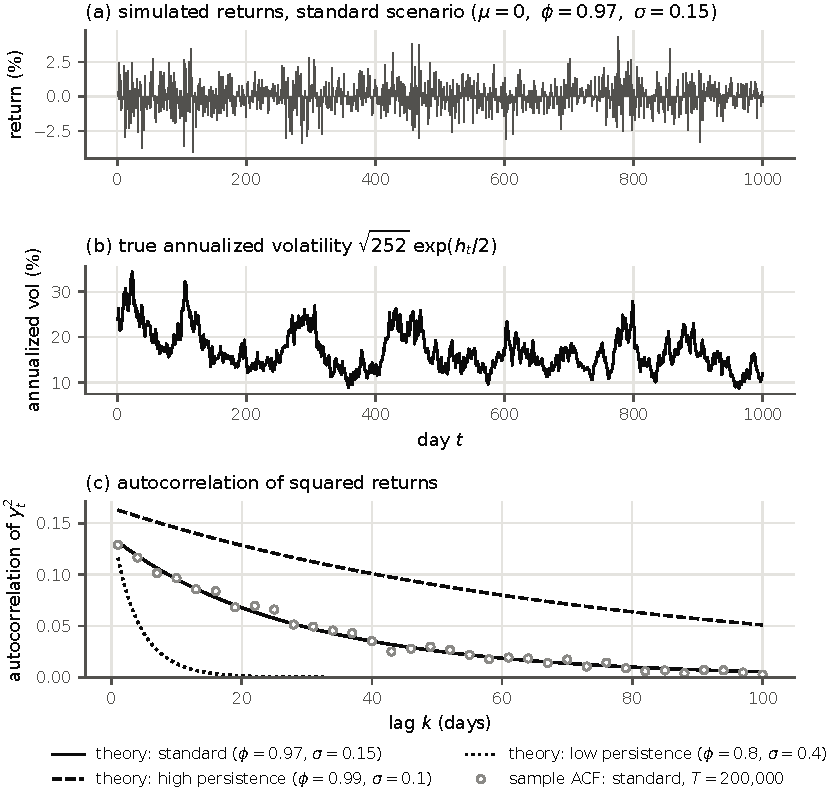
\includegraphics[width=\linewidth]{figures/fig1_sv_illustration.pdf}
  \caption{基本 SV モデルの例。(a) 標準シナリオ（$\mu = 0$、$\phi = 0.97$、$\sigma = 0.15$）から生成したリターン $y_t$（$T = 1{,}000$）。
    (b) その真の年率ボラティリティ $\sqrt{252}\exp(h_t/2)$。
    (c) 二乗リターンの自己相関。線は \cref{eq:sv-acf} による理論値（実線：標準、破線：高持続 $\phi = 0.99$、$\sigma = 0.10$、点線：低持続 $\phi = 0.8$、$\sigma = 0.4$）、
    白丸は標準シナリオの $T = 200{,}000$ の合成データから計算した標本自己相関（3 ラグごとに表示）。}
  \label{fig:sv-illustration}
\end{figure}

\cref{tab:sv-properties} は、合成データの 3 つのシナリオと、実データ（\cref{sec:empirical} の ETF 2 銘柄を NUTS で推定した事後平均）について、これらの量をまとめたものである。
合成データのシナリオは、いずれも $s \approx 0.6$〜$0.7$、尖度 4.4〜5.0 と裾の厚さは同程度だが、ショックの半減期が 3 日から 69 日まで大きく異なるように選んでいる。
実データの推定値は、$\phi$ が 0.86〜0.89 と合成データの標準シナリオより低く、$\sigma$ が 0.38〜0.46 と大きい。
その結果、半減期は 4〜6 日と短く、尖度は 6 を超える。
これは、推定に使った約 2 年の期間に 2025 年 4 月の急変動が含まれていることの影響が大きいと考えられる（\cref{sec:empirical} で改めて議論する）。

\begin{table}[tbp]
  \centering
  \caption{基本 SV モデルの定常的な性質。
    $s = \sqrt{\sigma^2/(1-\phi^2)}$ は対数ボラティリティの定常標準偏差、尖度は \cref{eq:sv-kurtosis} の $3e^{s^2}$、
    半減期は $\log 0.5 / \log\phi$、年率ボラの 95\% 範囲は定常分布 $h_t \sim \Normal(\mu, s^2)$ のもとでの $\sqrt{252}\exp(h_t/2)$ の 2.5\%・97.5\% 点。
    実データの行は \cref{sec:empirical} の NUTS による事後平均を代入した値。}
  \label{tab:sv-properties}
  \small
  \begin{tabular}{lrrrrrrr}
\toprule
 & $\mu$ & $\phi$ & $\sigma$ & $s$ & 尖度 & 半減期[日] & 年率ボラの95\%範囲[\%] \\
\midrule
合成：標準 & 0.00 & 0.970 & 0.150 & 0.617 & 4.39 & 22.8 & 8.7〜29.1 \\
合成：高持続 & 0.00 & 0.990 & 0.100 & 0.709 & 4.96 & 69.0 & 7.9〜31.8 \\
合成：低持続 & 0.00 & 0.800 & 0.400 & 0.667 & 4.68 & 3.1 & 8.3〜30.5 \\
\addlinespace
実データ：1321 & 0.61 & 0.889 & 0.384 & 0.840 & 6.07 & 5.9 & 9.5〜49.0 \\
実データ：1306 & 0.07 & 0.855 & 0.455 & 0.877 & 6.48 & 4.4 & 7.0〜38.9 \\
\bottomrule
\end{tabular}

\end{table}

\subsection{拡張 1：レバレッジ効果}\label{sec:model-leverage}

株式市場では、株価が下落した後にボラティリティが上昇しやすいという非対称性がよく知られており、\textbf{レバレッジ効果}と呼ばれる。
名前の由来は、株価が下がると企業の負債・自己資本比率（財務レバレッジ）が上がり、株式のリスクが高まるという説明である \parencite{christie1982}。
ほかにも、ボラティリティの上昇が予想されると投資家がより高いリスクプレミアムを求めて株価が下がる、という逆向きの因果による説明もある。
いずれの説明が正しいにせよ、下落局面でボラティリティが高まることは、VaR や ES のように損失側の裾を問題にする指標に直接影響するので、実務上重要な性質である。

SV モデルでは、レバレッジ効果を観測のショック $\varepsilon_t$ と状態のショック $\eta_t$ の相関として表す。本稿では
\begin{equation}
  y_t = \exp(h_t/2)\,\varepsilon_t, \qquad
  h_{t+1} = \mu + \phi\,(h_t - \mu) + \sigma\,\eta_t, \qquad
  \begin{pmatrix} \varepsilon_t \\ \eta_t \end{pmatrix} \sim \Normal\!\left( \begin{pmatrix} 0 \\ 0 \end{pmatrix}, \begin{pmatrix} 1 & \rho \\ \rho & 1 \end{pmatrix} \right)
  \label{eq:sv-leverage}
\end{equation}
とし、$\rho \in (-1, 1)$ を新たなパラメータとする（$t = T$ の $\varepsilon_T$ に対応する $\eta_T$ はモデルに現れない）。
$\rho < 0$ であれば、今日のリターンが負（$\varepsilon_t < 0$）のときに明日の対数ボラティリティへのショック $\eta_t$ が正になりやすく、レバレッジ効果が表される。

ここで重要なのは\textbf{時点の取り方}である。
\cref{eq:sv-leverage} では、今日の観測ショック $\varepsilon_t$ が、\textbf{明日}の対数ボラティリティ $h_{t+1}$ を動かすショック $\eta_t$ と相関する
\parencite{harvey1996,omori2007}。
これに対して、今日の $\varepsilon_t$ と今日の $h_t$ を動かすショック $\eta_{t-1}$ を相関させる定式化もある \parencite{jacquier2004}。
\textcite{yu2005} は二つの定式化を比較し、前者では $y_t$ がマルチンゲール差分（過去の情報のもとで条件付き平均が 0）になり、$\rho$ がレバレッジ効果の大きさとして素直に解釈できるのに対し、
後者ではそうならないことを示して、前者を支持している。本稿も前者を採用する。

実装と後の議論のために、\cref{eq:sv-leverage} を二通りの条件付き分布で書き直しておく。
二変量正規分布の条件付き分布の公式から、$\eta_t$ を与えたときの $\varepsilon_t$ は $\Normal(\rho\,\eta_t,\ 1-\rho^2)$ に、
$\varepsilon_t$ を与えたときの $\eta_t$ は $\Normal(\rho\,\varepsilon_t,\ 1-\rho^2)$ に従う。
\begin{enumerate}[label=(\alph*)]
  \item \textbf{観測を状態で条件付ける形}：$h_t$ と $h_{t+1}$ が分かれば $\eta_t = \{h_{t+1} - \mu - \phi(h_t - \mu)\}/\sigma$ が決まるので、
    \begin{equation}
      y_t \mid h_t, h_{t+1} \sim \Normal\!\left(\rho\, e^{h_t/2}\, \eta_t,\ (1-\rho^2)\, e^{h_t}\right) \quad (t < T), \qquad
      y_T \mid h_T \sim \Normal(0,\ e^{h_T}).
      \label{eq:sv-leverage-obs}
    \end{equation}
    $h_{1:T}$ の周辺分布は基本 SV と同じ AR(1) 過程であり（$\eta_t$ の周辺分布は $\Normal(0, 1)$ のまま）、
    同時分布は $p(h_{1:T} \mid \theta) \prod_{t} p(y_t \mid h_t, h_{t+1}, \theta)$ と分解できる。
    本稿の実装（尤度の計算）はこの形を使う。
  \item \textbf{状態を観測で条件付ける形}：今日のリターン $y_t$ が分かれば $\varepsilon_t = y_t\, e^{-h_t/2}$ が決まるので、
    \begin{equation}
      h_{t+1} \mid h_t, y_t \sim \Normal\!\left(\mu + \phi\,(h_t - \mu) + \rho\,\sigma\, y_t\, e^{-h_t/2},\ \ \sigma^2 (1-\rho^2)\right).
      \label{eq:sv-leverage-state}
    \end{equation}
    明日の対数ボラティリティは、基本 SV の AR(1) の予測に、今日の標準化リターンに比例する項 $\rho\sigma\, y_t e^{-h_t/2}$ を足したものになる。
    $\rho < 0$ なら、大きな下落の翌日には対数ボラティリティが押し上げられる。
    同時に、予測の不確実性は $\sigma^2$ から $\sigma^2(1-\rho^2)$ に小さくなる（今日のリターンが明日のボラティリティの情報を含むため）。
    この形は、1 期先の予測（\cref{sec:model-predictive}）と、\cref{sec:family} で条件付き構造化変分族をレバレッジ SV に拡張するときに使う。
\end{enumerate}

\subsection{拡張 2：$t$ 分布の誤差}\label{sec:model-t}

基本 SV モデルは、ボラティリティの変動によって周辺分布の裾を厚くするが、各日の条件付き分布は正規分布のままである。
しかし実際のリターンには、その日のボラティリティの水準から見ても極端に大きな変動（例えば突然のニュースによる急落）が含まれることがある。
これを表すために、観測ショック $\varepsilon_t$ を、分散が 1 になるように基準化した自由度 $\nu$ の $t$ 分布に置き換える \parencite{chib2002,jacquier2004}。
\begin{equation}
  y_t = \exp(h_t/2)\,\varepsilon_t, \qquad \varepsilon_t = \sqrt{\frac{\nu-2}{\nu}}\; u_t, \qquad u_t \sim t_\nu, \qquad \nu > 2.
  \label{eq:sv-t}
\end{equation}
自由度 $\nu$ の $t$ 分布の分散は $\nu/(\nu-2)$ なので、係数 $\sqrt{(\nu-2)/\nu}$ を掛けると $\varepsilon_t$ の分散は 1 になる。
この基準化により、$h_t$ は基本 SV と同じく「日次分散の対数」という意味を保ち、$\nu$ は分散を変えずに裾の厚さだけを表すパラメータになる。
基準化には分散が有限であること、すなわち $\nu > 2$ が必要である。
状態方程式 \cref{eq:sv-state,eq:sv-init} は基本 SV と同じである。

観測の対数尤度は
\[
  \log p(y_t \mid h_t, \nu) = \log \Gamma\!\left(\tfrac{\nu+1}{2}\right) - \log \Gamma\!\left(\tfrac{\nu}{2}\right) - \frac{1}{2}\log\{\pi(\nu-2)\}
    - \frac{h_t}{2} - \frac{\nu+1}{2} \log\!\left(1 + \frac{y_t^2\, e^{-h_t}}{\nu - 2}\right)
\]
である。
$t$ 分布は、正規分布の分散を逆ガンマ分布に従って確率的に変えた混合分布として
$\varepsilon_t = \sqrt{(\nu-2)\lambda_t/\nu}\; z_t$、$z_t \sim \Normal(0,1)$、$\lambda_t \sim \mathrm{InvGamma}(\nu/2,\ \nu/2)$
とも書ける。MCMC ではこの表現で $\lambda_t$ を潜在変数として加えることが多いが、本稿では $\lambda_t$ を積分消去した上の密度をそのまま使う
（変分推論では、潜在変数を増やさずに直接扱える方が素直だからである）。

$t$ 誤差の SV モデルの尖度は、$\nu > 4$ のとき
\[
  \kappa = 3\,\frac{\nu-2}{\nu-4}\; e^{s^2}
\]
であり、ボラティリティの変動による部分 $e^{s^2}$ と、各日の条件付き分布の裾による部分 $(\nu-2)/(\nu-4)$ の積になる。
二つの拡張の役割を整理すると、基本 SV がボラティリティの「ゆっくりした」変動を、$t$ 誤差がボラティリティの水準では説明できない「単発の」大きな変動を担当する、という分担になる。
どちらがデータの裾の厚さをどれだけ説明するかは、推定してみて初めて分かる（実データでは $\nu$ の事後平均が 20〜25 と大きく、裾の厚さはほぼボラティリティの変動で説明された。\cref{sec:empirical}）。

なお本稿では、レバレッジ効果と $t$ 誤差を同時に持つモデルは扱わない。
両者を組み合わせるには、$\varepsilon_t$ と $\eta_t$ の同時分布を（二変量正規分布ではなく）別の形で定める必要があり、モデルと推定の両面で議論が増えるためである。

\subsection{事前分布}\label{sec:model-prior}

ベイズ推定では、パラメータ $\theta$ に事前分布を置く。本稿で使う事前分布を \cref{tab:priors} にまとめる。

\begin{table}[tbp]
  \centering
  \caption{事前分布と、その平均・95\% 区間（2.5\%・97.5\% 点）。$\sigma$ の事前分布は半正規分布を標準とし、逆ガンマ分布（$\sigma^2$ に対する）は感度分析（\cref{app:settings}）でのみ使う。}
  \label{tab:priors}
  \small
  \begin{tabular}{llrl}
\toprule
パラメータ & 事前分布 & 事前平均 & 95\% 区間 \\
\midrule
$\mu$ & $\Normal(0,\ 10^2)$ & 0.0 & [-19.6,\ 19.6] \\
$\phi$ & $(\phi+1)/2 \sim \mathrm{Beta}(20,\ 1.5)$ & 0.860 & [0.588,\ 0.989] \\
$\sigma$ & $\mathrm{HalfNormal}(1)$（標準） & 0.798 & [0.031,\ 2.241] \\
$\sigma$ & $\sigma^2 \sim \mathrm{InvGamma}(2.5,\ 0.025)$（感度分析） & 0.119 & [0.062,\ 0.245] \\
$\rho$ & $\mathrm{Uniform}(-1,\ 1)$ & 0.000 & [-0.95,\ 0.95] \\
$\nu$ & $\nu-2 \sim \mathrm{Gamma}(2,\ 0.1)$ & 22.0 & [4.4,\ 57.7] \\
\bottomrule
\end{tabular}

\end{table}

\begin{itemize}
  \item $\mu \sim \Normal(0, 10^2)$：\% 単位では $\mu$ は $-1$〜$2$ 程度なので、標準偏差 10 は実質的に情報を持たない（弱情報の）事前分布である。
  \item $(\phi + 1)/2 \sim \mathrm{Beta}(20, 1.5)$：\textcite{kim1998} 以来、SV モデルで標準的に使われている事前分布である。
    $\phi$ を $(-1, 1)$ に収めつつ、日次データで典型的な高い持続性に事前の重みを置く（事前平均 0.86、95\% 区間 $[0.59, 0.99]$）。
    実データの推定値（0.86〜0.89）はこの区間の中央付近にある。一方、高持続シナリオの真値 0.99 は区間の上端にあたり、事前分布が $\phi$ をわずかに下に引く方向に働く。
  \item $\sigma \sim \mathrm{HalfNormal}(1)$（半正規分布）：$\sigma^2$ に $\chi^2_1$ 分布（形状 1/2 のガンマ分布）を置くことと同じであり、
    \textcite{kastner2014} でも使われている。
    \textcite{kim1998} は $\sigma^2$ に逆ガンマ分布 $\mathrm{InvGamma}(2.5,\ 0.025)$ を置いたが、逆ガンマ分布は $\sigma = 0$ の近くで密度が 0 になり、$\sigma$ を 0 から遠ざける方向に働く。
    また \cref{tab:priors} のとおり、この逆ガンマ分布は $\sigma$ の 95\% 区間が $[0.06, 0.25]$ と狭く、実データの推定値（0.38〜0.46）はその外側にある。
    半正規分布は $\sigma = 0$ の近くでも正の密度を持ち、かつ 0.03〜2.2 という広い範囲を覆うので、本稿ではこちらを標準とする。
    逆ガンマ分布は合成データでの感度分析にのみ使い、提案手法の推定結果が事前分布の選び方でほとんど変わらないことを確認している（\cref{app:settings}）。
  \item $\rho \sim \mathrm{Uniform}(-1, 1)$：レバレッジの向きと大きさについて事前に特定の値を仮定しない。
  \item $\nu - 2 \sim \mathrm{Gamma}(2,\ 0.1)$（形状 2、レート 0.1）：自由度の事前分布として広く使われる $\mathrm{Gamma}(2, 0.1)$ \parencite{juarez2010} を、
    基準化に必要な $\nu > 2$ を満たすように 2 だけずらしたものである。事前平均は 22、95\% 区間は $[4.4, 57.7]$ で、裾の厚い分布（$\nu \approx 5$）から正規分布に近い分布（$\nu > 30$）までを覆う。
\end{itemize}

事前分布は、データが十分にあれば推定結果にほとんど影響しないが、本稿の実データのように系列が短い（約 500 日）場合には無視できないことがある。
とくに $\nu$ は裾の観測が少ないと事後分布が事前分布からあまり動かず、実データでの $\nu$ の推定値はこの点を割り引いて読む必要がある（\cref{sec:empirical}）。

\subsection{尤度が解析的に書けない理由と事後分布}\label{sec:model-likelihood}

パラメータ $\theta$ の尤度は、\cref{eq:sv-joint} を潜在変数 $h_{1:T}$ について積分した
\begin{equation}
  p(y_{1:T} \mid \theta) = \int p(y_{1:T} \mid h_{1:T})\, p(h_{1:T} \mid \theta)\, dh_{1:T}
  \label{eq:sv-marginal}
\end{equation}
である。これは $T$ 次元の積分であり、閉じた形では計算できない。

もし観測方程式が $h_t$ について線形で、誤差が正規分布であれば、\cref{eq:sv-marginal} はカルマンフィルタによって $O(T)$ の計算量で厳密に計算できる。
SV モデルの観測方程式は、$y_t$ の分散が $e^{h_t}$ という形で $h_t$ に非線形に依存しており、この条件を満たさない。
両辺を二乗して対数をとると
\[
  \log y_t^2 = h_t + \log \varepsilon_t^2
\]
と $h_t$ について線形になるが、誤差 $\log \varepsilon_t^2$ は $\log \chi^2_1$ 分布という左に長い裾を持つ非正規分布に従う（平均 $\approx -1.27$、分散 $\pi^2/2 \approx 4.93$）。
これを正規分布で置き換えてカルマンフィルタを使うのが疑似最尤法（QML）\parencite{harvey1994} であり、
$\log \chi^2_1$ 分布を正規分布の混合で精度よく近似して MCMC に組み込んだのが \textcite{kim1998} である。

この変形は、SV モデルの推定が難しいもう一つの理由も教えてくれる。
1 日分の観測 $\log y_t^2$ に含まれる $h_t$ の情報は、分散 4.93 という大きなノイズに埋もれている。
一方、$h_t$ 自体の変動の大きさは定常分散 $s^2$ でおよそ 0.4〜0.8 にすぎない（\cref{tab:sv-properties}）。
つまり 1 日の観測だけでは $h_t$ はほとんど決まらず、\textbf{$h_t$ の推定は、前後の多くの日の観測を AR(1) の構造を通じて平滑化することで初めて可能になる}。
これは、$h_t$ の事後分布で隣り合う日どうしが強く相関することを意味しており、\cref{sec:family} で平均場近似が失敗する理由そのものである。

ベイズ推定では、積分 \cref{eq:sv-marginal} を直接計算する代わりに、潜在変数 $h_{1:T}$ もパラメータと一緒に未知数として扱い、同時事後分布
\begin{equation}
  p(\theta, h_{1:T} \mid y_{1:T}) \;\propto\; p(\theta)\; p(h_{1:T} \mid \theta)\; p(y_{1:T} \mid h_{1:T}, \theta)
  \label{eq:sv-posterior}
\end{equation}
を考える。右辺は \cref{eq:sv-loglik} などの初等的な関数の積なので、正規化定数を除けばいつでも計算できる。
求めたいのは $\theta$ と $h_{1:T}$ の事後分布（の要約）であり、その次元は $T + k$（$k$ は大域パラメータの数で、基本 SV で 3、拡張モデルで 4）である。
本稿の実データ（$T = 485$）でも約 500 次元、10 年分の日次データなら約 2,500 次元になる。
\cref{sec:inference} で述べる MCMC と変分推論は、いずれもこの高次元の事後分布 \cref{eq:sv-posterior} を扱う方法である。

なお、観測の対数尤度 \cref{eq:sv-loglik} は $h_t$ について凹関数である（2 階微分が $-y_t^2 e^{-h_t}/2 \leq 0$）。
$t$ 誤差の場合も、$a_t = y_t^2/(\nu-2)$、$u_t = a_t e^{-h_t}$ とおくと 2 階微分は $-\frac{\nu+1}{2}\,\frac{u_t}{(1+u_t)^2} \leq 0$ で、やはり凹である。
AR(1) の事前分布も $h_{1:T}$ について凹（対数が二次形式）なので、$\theta$ を固定したときの $h_{1:T}$ の事後分布は単峰で、正規分布による近似がよく効く。
二つのモデルの曲率を比べると、正規誤差では大きなリターン $y_t$ ほど曲率 $y_t^2 e^{-h_t}/2$ が際限なく大きくなり、1 日の極端なリターンが $h_t$ を強く引き寄せる。
$t$ 誤差では曲率が $(\nu+1)/8$ 以下に抑えられ、極端なリターンの影響が自動的に割り引かれる（頑健になる）。
また、リターンがちょうど 0 の日（売買が少ない銘柄などで生じる）は、正規誤差の対数尤度が $-h_t/2$ だけになり単独では $h_t \to -\infty$ を好むが、AR(1) の事前分布が $h_t$ を前後の日の水準に引き留めるので、推定上の問題にはならない。

\subsection{事後分布の構造：三重対角の精度行列}\label{sec:model-structure}

\cref{sec:family} で変分族を設計するために、事後分布 \cref{eq:sv-posterior} の構造をもう少し詳しく見ておく。
鍵になるのは、正規分布の\textbf{精度行列}（共分散行列の逆行列）である。
多変量正規分布では、精度行列の $(i, j)$ 成分が 0 であることと、「他のすべての変数を与えたとき、$i$ 番目と $j$ 番目の変数が条件付き独立であること」が同値になる。
したがって、変数間の条件付き独立性が多ければ精度行列は疎（0 の多い行列）になる。

\paragraph{AR(1) の事前分布の精度行列}
\cref{eq:sv-state,eq:sv-init} の定常 AR(1) 過程では、$h_t$ は直前の $h_{t-1}$ と直後の $h_{t+1}$ を与えれば、それ以外の日と条件付き独立である。
実際、$p(h_{1:T} \mid \theta)$ の対数は $h_{1:T}$ の二次形式であり、$h - \mu\mathbf{1}$ についての精度行列は
\begin{equation}
  Q_{\mathrm{AR}}(\phi, \sigma) = \frac{1}{\sigma^2}
  \begin{pmatrix}
    1      & -\phi    &        &        &        \\
    -\phi  & 1+\phi^2 & -\phi  &        &        \\
           & \ddots   & \ddots & \ddots &        \\
           &          & -\phi  & 1+\phi^2 & -\phi \\
           &          &        & -\phi  & 1
  \end{pmatrix}
  \label{eq:ar1-precision}
\end{equation}
という\textbf{三重対角行列}になる（空白の成分は 0）。
左上の成分は、定常分布の精度 $(1-\phi^2)/\sigma^2$ と、$h_2$ の式から来る $\phi^2/\sigma^2$ の和として $1/\sigma^2$ になる。
共分散行列（$\mathrm{Cov}(h_s, h_t) = s^2 \phi^{|s-t|}$）は密な行列であるのに、精度行列はこのように疎である。

\paragraph{$\theta$ を固定したときの $h$ の事後分布}
次に、$\theta$ を固定して $h_{1:T}$ の事後分布 $p(h_{1:T} \mid y_{1:T}, \theta)$ を考える。
その対数は、AR(1) の事前分布の対数（三重対角の二次形式）と、各日の観測の対数尤度の和 $\sum_t \log p(y_t \mid h_t)$ からなる。
後者は $h_t$ ごとに分かれた和なので、$h_{1:T}$ についてのヘッセ行列（2 階微分の行列）は\textbf{対角行列}である。
したがって、事後分布の最頻値 $\hat h$ のまわりで二次近似（ラプラス近似）をすると、近似した正規分布の精度行列は
\begin{equation}
  Q_{\mathrm{AR}}(\phi, \sigma) + \diag\!\left( \frac{y_1^2}{2}\,e^{-\hat h_1}, \dots, \frac{y_T^2}{2}\,e^{-\hat h_T} \right)
  \label{eq:laplace-precision}
\end{equation}
となり、やはり三重対角である。
つまり、$\theta$ を与えたときの $h$ の事後分布は、「AR(1) の事前分布」に「各日ごとの正規分布の形をした情報」を掛け合わせたもので、よく近似できる。
\cref{sec:family} の条件付き構造化変分族は、まさにこの形（各日の情報の位置と精度を変分パラメータとして最適化する）を変分族として採用したものである。

$t$ 誤差のモデルでも観測の対数尤度は $h_t$ ごとに分かれるので、構造は同じである。
レバレッジ SV では、\cref{eq:sv-leverage-obs} のとおり $y_t$ の尤度が $h_t$ と $h_{t+1}$ の両方に依存するが、依存するのは隣り合う日の組だけなので、
ヘッセ行列への寄与は $(t, t)$、$(t, t+1)$、$(t+1, t+1)$ 成分に限られ、\textbf{三重対角の帯構造は保たれる}（ただし、各日の寄与が凹であるとは限らない）。

三重対角の精度行列を持つ正規分布は、コレスキー分解・前進代入・後退代入をすべて $O(T)$ の計算量で行える。
したがって、密度の計算・サンプリング・エントロピーの計算をすべて $O(T)$ で行える。
これは、MCMC で状態を一括してサンプリングするために \textcite{chan2009} が使った性質であり、本稿では変分族の側で利用する（\cref{sec:family}）。

\paragraph{パラメータと状態の事後的な依存}
同時事後分布 \cref{eq:sv-posterior} では、$\theta$ と $h_{1:T}$ も互いに強く依存する。
\begin{itemize}
  \item \textbf{$\sigma$ と $h$ の滑らかさ}：\cref{eq:laplace-precision} のとおり、$h$ の事後分布の精度行列の大部分は $1/\sigma^2$ に比例する。
    $\sigma$ が小さいと考えるなら $h$ の経路は滑らかでなければならず、$\sigma$ が大きいと考えるなら $h$ は日々大きく動いてよい。
    $\sigma$ の不確実性を正しく表すには、$h$ の経路の滑らかさが $\sigma$ に連動して変わる必要がある。
  \item \textbf{$\mu$ と $h$ の水準}：$\mu$ を大きく見積もるなら、$h$ 全体も上に動く。
  \item \textbf{$\mu$ と $\phi$}：$\mu$ は $h_t$ が戻っていく先の水準なので、$h_t$ の平均回帰が速い（$\phi$ が小さい）ほどよく決まり、$\phi$ が 1 に近いほど決まりにくい。
    AR(1) 過程の標本平均の分散がおよそ $\sigma^2 / \{(1-\phi)^2 T\}$ であることからも分かるように、$\phi$ が 1 に近づくと $\mu$ の事後分布の幅は急速に広がる。
    例えば実データの 1321 の推定値（$\phi \approx 0.89$、$\sigma \approx 0.38$、$T = 485$）では、この式から $\mu$ の不確実性は標準偏差で約 0.16 と見積もられ、NUTS による事後標準偏差 0.21 と同程度の大きさになる。
    この結果、$(\mu, \phi)$ の同時事後分布は、$\phi$ が大きいところほど $\mu$ の方向に広がる「バナナ型」の形になり、正規分布ではうまく表せない。
\end{itemize}
これらの依存は、$\theta$ と $h$ を独立とみなす変分族では表現できない。
\cref{sec:family,sec:synthetic} で見るように、とくに $\sigma$ と $h$ の依存を無視すると、$\sigma$ の不確実性が大きく過小評価される。

\subsection{パラメータ化：中心化と非中心化}\label{sec:model-param}

同じ SV モデルでも、潜在変数を何に取るか（\textbf{パラメータ化}）によって、推定のしやすさが大きく変わる。
ここまでの定式化のように $h_{1:T}$ そのものを潜在変数とするものを\textbf{中心化パラメータ化}と呼ぶ。
これに対して、標準化した
\[
  x_t = \frac{h_t - \mu}{\sigma}, \qquad
  x_1 \sim \Normal\!\left(0, \frac{1}{1-\phi^2}\right), \quad x_{t+1} = \phi\, x_t + \eta_t, \qquad h_t = \mu + \sigma\, x_t
\]
を潜在変数とするものを\textbf{非中心化パラメータ化}と呼ぶ。
二つは同じ確率モデルの異なる表現であり、事後分布から計算される $h_t$ や $\theta$ の分布は（推定が正確であれば）一致する。
違うのは、推定アルゴリズムから見た事後分布の「形」である。
中心化では、事前分布の段階で $h$ が $\mu$・$\sigma$ に依存する（$\mu$ と $\sigma$ が $h$ の水準と滑らかさを決める）。
非中心化では、事前分布の段階では $x$ と $(\mu, \sigma)$ が独立になり、依存は観測の尤度を通じてだけ生じる。

一般に、データが潜在変数についての情報を多く含むときは中心化が、少ないときは非中心化が、MCMC の効率の点で有利になることが知られている \parencite{papaspiliopoulos2007}。
SV モデルでは、どちらが有利かがパラメータの値やデータによって変わり、
\textcite{kastner2014} の ASIS は、二つのパラメータ化を交互に使うことで両方の長所を取り入れる方法である。

本稿の予備実験では、持続性の高いシナリオ（$\phi = 0.99$、$T = 1{,}000$）で、非中心化の NUTS は $\mu$ がほとんど混合せず（ESS は約 10、$\hat R = 1.66$）、
中心化の NUTS では $\mu$ の ESS が約 3,000 と良好だった（一方で、$\sigma$ の ESS は約 80 と低めだった）。
そこで本稿では、「正解」として使う NUTS には中心化パラメータ化を採用し、混合の悪さを補うために反復を長くとる（\cref{sec:synthetic}）。

変分推論でも、パラメータ化の選択は結果に影響しうる。
平均場近似や、$\theta$ と $h$ を独立とする構造化近似では、どちらのパラメータ化で変分族を当てるかによって近似の結果が変わる（\cref{app:settings}）。
一方、\cref{sec:family} の条件付き構造化変分族は、$\theta$ を固定すると $h = \mu + \sigma x$ がアフィン変換であることから、\textbf{どちらのパラメータ化を使っても同じ分布族になる}。
パラメータ化という調整項目を一つ減らせることは、システムとして運用するうえでの利点でもある。

\subsection{1 期先の予測分布と VaR}\label{sec:model-predictive}

最後に、\cref{sec:empirical} の VaR のバックテストで使う 1 期先の予測分布を定義する。
時点 $T$ までのデータ $y_{1:T}$ をもとにした翌日のリターン $y_{T+1}$ の予測分布は、
\begin{equation}
  p(y_{T+1} \mid y_{1:T}) = \int p(y_{T+1} \mid h_{T+1}, \theta)\; p(h_{T+1} \mid h_T, y_T, \theta)\; p(\theta, h_T \mid y_{1:T})\; d\theta\, dh_T\, dh_{T+1}
  \label{eq:predictive}
\end{equation}
である。ここで $p(\theta, h_T \mid y_{1:T})$ は同時事後分布 \cref{eq:sv-posterior} の $(\theta, h_T)$ についての周辺分布であり、
最終時点 $h_T$ については、これは「時点 $T$ までの情報で見た今日の対数ボラティリティの分布」（フィルタリング分布）に一致する。
$p(h_{T+1} \mid h_T, y_T, \theta)$ は、基本 SV と $t$ 誤差のモデルでは状態方程式 \cref{eq:sv-state} そのもの（$y_T$ には依存しない）、
レバレッジ SV では \cref{eq:sv-leverage-state} である。
レバレッジ SV では、今日のリターン $y_T$ が負で大きいほど翌日のボラティリティの予測が上がり、VaR が保守的になる。

実際の計算では、MCMC のサンプル、または変分分布から生成したサンプル $(\theta^{(s)}, h_T^{(s)})$、$s = 1, \dots, S$ を使う。
各サンプルについて $h_{T+1}^{(s)}$ を状態方程式から 1 つ生成すると、予測分布は
\[
  p(y_{T+1} \mid y_{1:T}) \approx \frac{1}{S} \sum_{s=1}^{S} p\!\left(y_{T+1} \mid h_{T+1}^{(s)}, \theta^{(s)}\right)
\]
という $S$ 個の正規分布（$t$ 誤差のモデルでは $t$ 分布）の混合で近似できる。
この混合分布は、パラメータの不確実性と今日・明日のボラティリティの不確実性をすべて反映しているので、単一の正規分布より裾が厚い。
有意水準 $\alpha$（本稿では 5\% と 1\%）の VaR は、この混合分布の下側 $\alpha$ 分位点、すなわち
\[
  \frac{1}{S} \sum_{s=1}^{S} F\!\left(q \mid h_{T+1}^{(s)}, \theta^{(s)}\right) = \alpha
\]
を満たす $q$ として計算する（$F$ は各成分の累積分布関数。$q$ は 1 次元の方程式なので二分法などで確実に解ける）。
本稿では VaR をリターンの分位点（負の値）として表し、実現リターンが VaR を下回った日を「超過」と数える。
また、予測分布の良さを分位点だけでなく分布全体で評価するために、実現値 $y_{T+1}^{\mathrm{obs}}$ での対数予測密度（対数予測スコア）
\[
  \log p(y_{T+1}^{\mathrm{obs}} \mid y_{1:T}) \approx \log \frac{1}{S} \sum_{s=1}^{S} p\!\left(y_{T+1}^{\mathrm{obs}} \mid h_{T+1}^{(s)}, \theta^{(s)}\right)
\]
も計算する（大きいほど良い）。
混合分布の密度と累積分布関数を直接計算するので、$y_{T+1}$ をさらに乱数で生成して分位点を求めるより、モンテカルロ誤差が小さい。
推定方法（NUTS か変分推論か、どの変分族か）の違いは、すべてサンプル $(\theta^{(s)}, h_T^{(s)})$ の分布の違いとして予測分布に反映される。
とくに、変分推論が $\theta$ や $h_T$ の不確実性を過小評価すると、予測分布の裾が薄くなり、VaR の超過が増えることになる。
